\section{Design and how to respect the \textit{open-closed-principle}}
One main purpose of the use of java and object-oriented programming is that the code is easily extended so
new features and functions can easily be added to an already working system. Nevertheless, one has to 
respect some rules of programming in order to benefit from this advantage, i.e. the use of design patterns.
In our \textit{MyFoodora} we used several of these patters which are explained in this section.
\subsection{Package Management}
\label{sub:package_management}

Having read the project requirements for the first time we figured out that there were several different 
parts which can be treated seperately. This logic sepration of different parts of the system was used 
to organize our packages as well as the division of the work for the two members of the group. The
following main packages exist in the project:
\begin{itemize}
	\item{system} Contains the main funtionalities of \textit{MyFoodora}.
	\item{user-management} Manages users of the systems and asseses functions to groups of users.
	\item{restaurant} Manages the creation of meals and singleItems and do the pricing.
	\item{commandLineTool} Adds a command line user interface to the system.
	\item{GUI} Adds a graphical user interface to the system.
	\item{several Test packages} According their name they provide test for the previous packages.
\end{itemize}

The following diagram shows the interaction of the first three packages (The interfaces and testings 
do obviously interact with all the other ones).

\begin{figure}[h]
	\centering
	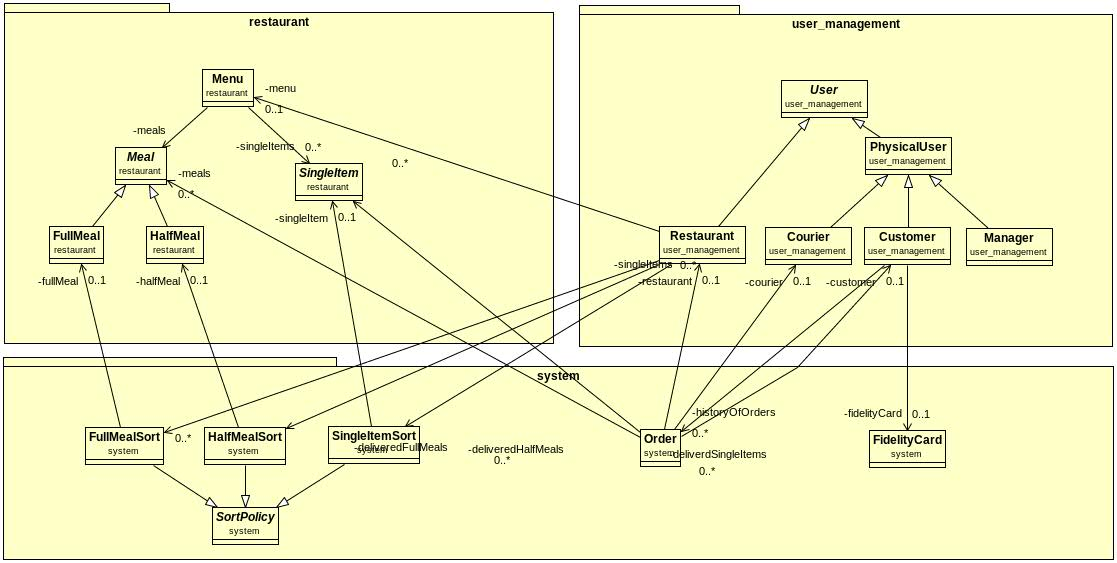
\includegraphics[width=0.8\linewidth]{./packages.jpg}
	\caption{Package-interactions}
	\label{fig:packages}
\end{figure}
